\begin{frame}{Benchmarks and What They Measure}

  {\centering\scriptsize
  \begin{tabular}{>{\raggedright\arraybackslash}p{1.6cm} >{\raggedright\arraybackslash}p{4.1cm} >{\raggedright\arraybackslash}p{3.0cm} >{\raggedright\arraybackslash}p{3.3cm}}
    \toprule
    \textbf{Benchmark} & \textbf{What it tests} & \textbf{Format} & \textbf{Metric} \\
    \midrule
    VQAv2\newline CVPR 2017 & Most questions get a similar photo with a different answer & about 1.1M image-question pairs on COCO & VQA accuracy \\
    \addlinespace[0.15em]
    TextVQA\newline CVPR 2019 & Reading text in photos: signs, brands, times & 45,336 questions on 28,408 images & VQA accuracy \\
    \addlinespace[0.15em]
    DocVQA\newline WACV 2021 & Reading document pages, where forms and tables carry meaning & 50,000 questions on 12,767 page images & ANLS: average normalized Levenshtein similarity \\
    \addlinespace[0.15em]
    MMMU\newline CVPR 2024 & College-level questions in 30 subjects and 30 image types & 11,550 questions, 94\% multiple choice & accuracy pooled over all questions (micro-average) \\
    \addlinespace[0.15em]
    MMBench\newline ECCV 2024 & 20 perception and reasoning abilities, in English and Chinese & 3,217 multiple-choice questions & CircularEval: right under every option rotation \\
    \addlinespace[0.15em]
    POPE\newline EMNLP 2023 & Object hallucination: naming objects that are not there & yes/no: ``Is there a \ldots{} in the image?'' & accuracy, F1, share of ``yes'' \\
    \addlinespace[0.15em]
    MMVP\newline CVPR 2024 & Details that CLIP encoders miss, such as orientation and counts & 300 two-option questions on 150 image pairs & pair accuracy: both questions right \\
    \bottomrule
  \end{tabular}\par}
  \vspace{0.4em}
  \begin{itemize}\footnotesize
    \item \textbf{ANLS} gives partial credit for near-miss strings. \textbf{CircularEval} repeats each question once per rotation of its options and needs every answer right: OpenFlamingo v2 drops from 36.7\% to 2.6\% on MMBench-dev.
  \end{itemize}
  \vspace{0.2em}
  {\scriptsize Goyal et al., \href{https://arxiv.org/abs/1612.00837v3}{arXiv:1612.00837v3}; Singh et al., \href{https://arxiv.org/abs/1904.08920v2}{arXiv:1904.08920v2}; Mathew et al., \href{https://arxiv.org/abs/2007.00398v3}{arXiv:2007.00398v3}; Yue et al., \href{https://arxiv.org/abs/2311.16502v4}{arXiv:2311.16502v4}; Liu et al., \href{https://arxiv.org/abs/2307.06281v5}{arXiv:2307.06281v5}, Table~2; Li et al., \href{https://arxiv.org/abs/2305.10355v3}{arXiv:2305.10355v3}; Tong et al., \href{https://arxiv.org/abs/2401.06209v2}{arXiv:2401.06209v2}.\par}
\end{frame}

\begin{frame}{Object Hallucination: POPE}
  \begin{columns}[T,onlytextwidth]
    \column{0.51\textwidth}
      \begin{itemize}\footnotesize\itemsep0.3em
        \item \textbf{Object hallucination:} naming objects absent from the image. POPE (Polling-based Object Probing Evaluation) asks ``Is there a $\langle\text{object}\rangle$ in the image?'', half about annotated objects (yes), half about absent ones (no).
        \item \textbf{Absent objects} are drawn at random (random), from the dataset's most frequent objects (popular), or from those that co-occur most with the objects present (adversarial).
        \item \textbf{Metrics} (``yes'' is positive): accuracy, precision, recall, F1, share of ``yes''. Always saying yes gives 50\% accuracy and F1 = 66.67.
        \item \textbf{It follows the instruction data} (mostly built on COCO): about half of hallucinated objects are among COCO's ten most frequent, over half among the ten that co-occur most with objects present. InstructBLIP, tuned on short public-dataset instructions, hallucinates least.
      \end{itemize}
    \column{0.47\textwidth}
      \centering
      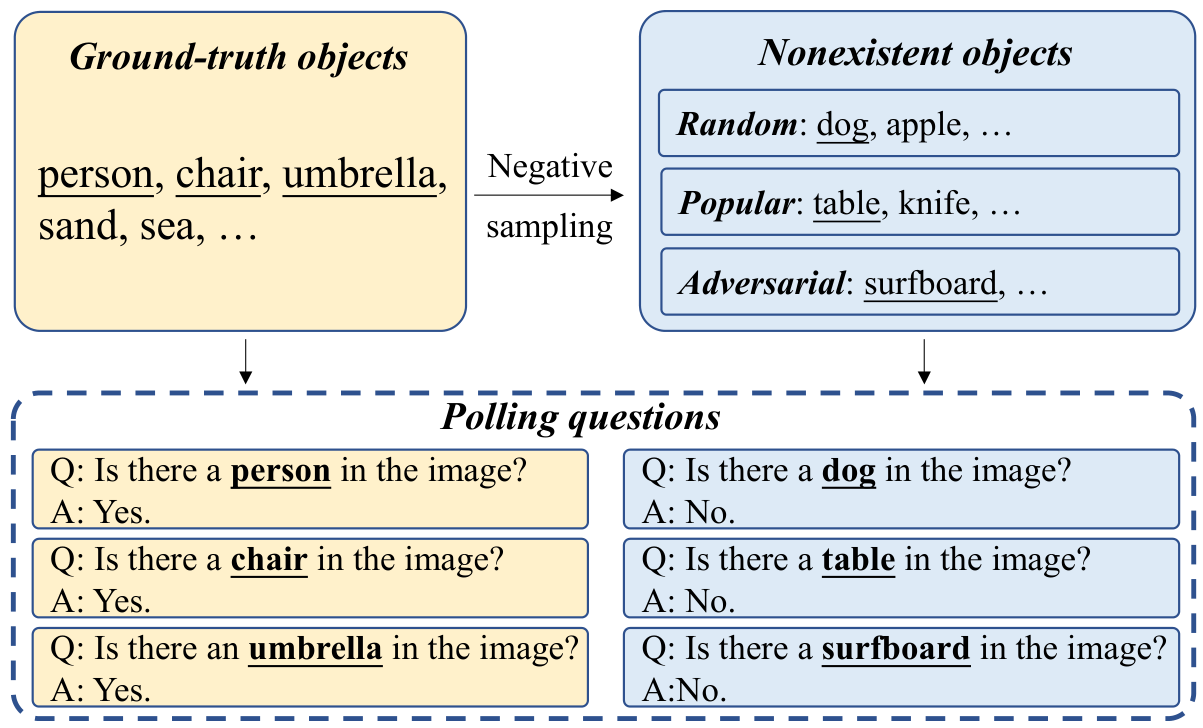
\includegraphics[width=\linewidth,height=0.40\textheight,keepaspectratio]{images/vision-language-models/pope_fig3_polling_pipeline.png}\\[0.2em]
      {\scriptsize Li et al., ``Evaluating Object Hallucination in Large Vision-Language Models,'' EMNLP 2023, \href{https://arxiv.org/abs/2305.10355v3}{arXiv:2305.10355v3}, Figure~3 (right part); Sections~3.2 and~4.3.\par}
      \vspace{0.5em}
      {\scriptsize\setlength{\tabcolsep}{3pt}
      \begin{tabular}{l l r r r}
        \toprule
         & & Random & Popular & Advers. \\
        \midrule
        LLaVA & accuracy & 54.43 & 52.43 & 50.77 \\
         & ``yes'' (\%) & 95.37 & 97.37 & 99.10 \\
        \addlinespace[0.2em]
        InstructBLIP & accuracy & 88.73 & 81.37 & 74.37 \\
         & ``yes'' (\%) & 55.20 & 62.57 & 68.97 \\
        \bottomrule
      \end{tabular}\par}
      \vspace{0.2em}
      {\scriptsize COCO val, 500 images, 6 probes each (Table~3).\par}
  \end{columns}
\end{frame}

\begin{frame}{Blind Spots Inherited from CLIP: MMVP}

  {\centering
  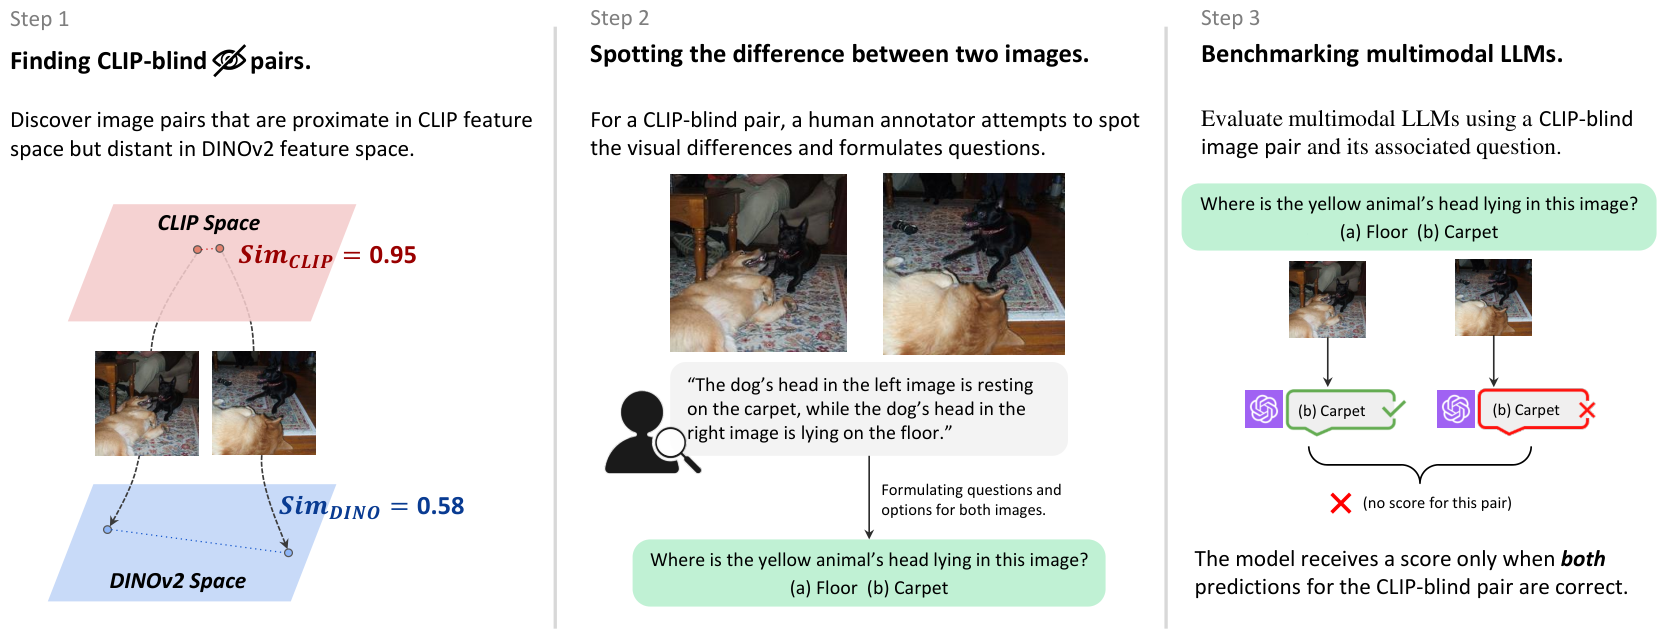
\includegraphics[width=\linewidth,height=0.66\textheight,keepaspectratio]{images/vision-language-models/mmvp_fig2_clip_blind_pairs.png}\\[0.2em]
  {\scriptsize Tong et al., ``Eyes Wide Shut? Exploring the Visual Shortcomings of Multimodal LLMs,'' CVPR 2024, \href{https://arxiv.org/abs/2401.06209v2}{arXiv:2401.06209v2}, Figure~2; thresholds from Section~2.1.\par}}
  \vspace{0.3em}
  \begin{itemize}\footnotesize
    \item \textbf{CLIP-blind pair:} two images with cosine similarity above 0.95 in CLIP ViT-L/14 but below 0.6 in DINOv2 ViT-L/14, a vision-only model that keeps more detail.
  \end{itemize}
\end{frame}

\begin{frame}{MMVP: Results and Failure Patterns}
  \begin{itemize}\itemsep0.6em
    \item \textbf{MMVP:} annotators wrote 300 two-option questions about the visible difference in 150 CLIP-blind pairs. A pair scores only if both answers are right, so guessing gives 25\%.
    \item \textbf{Results:} humans 95.7\%; Gemini 40.7\%, GPT-4V (GPT-4 with image input) 38.7\%; LLaVA-1.5 24.7\%, InstructBLIP 16.7\%, LLaVA (336 px) 6.0\%. Every other model tested is below chance.
    \item \textbf{Nine failure patterns,} among them orientation, counting and viewpoint: CLIP features favor high-level semantics over detail, the image-side twin of the bag-of-words behavior.
  \end{itemize}
  \vspace{0.6em}
  {\scriptsize Tong et al., \href{https://arxiv.org/abs/2401.06209v2}{arXiv:2401.06209v2}, Sections~2.2, 2.3 and~3.1, Figure~4.\par}
\end{frame}

\begin{frame}{Mixture of Features (MoF): CLIP Plus DINOv2}
  \centering
  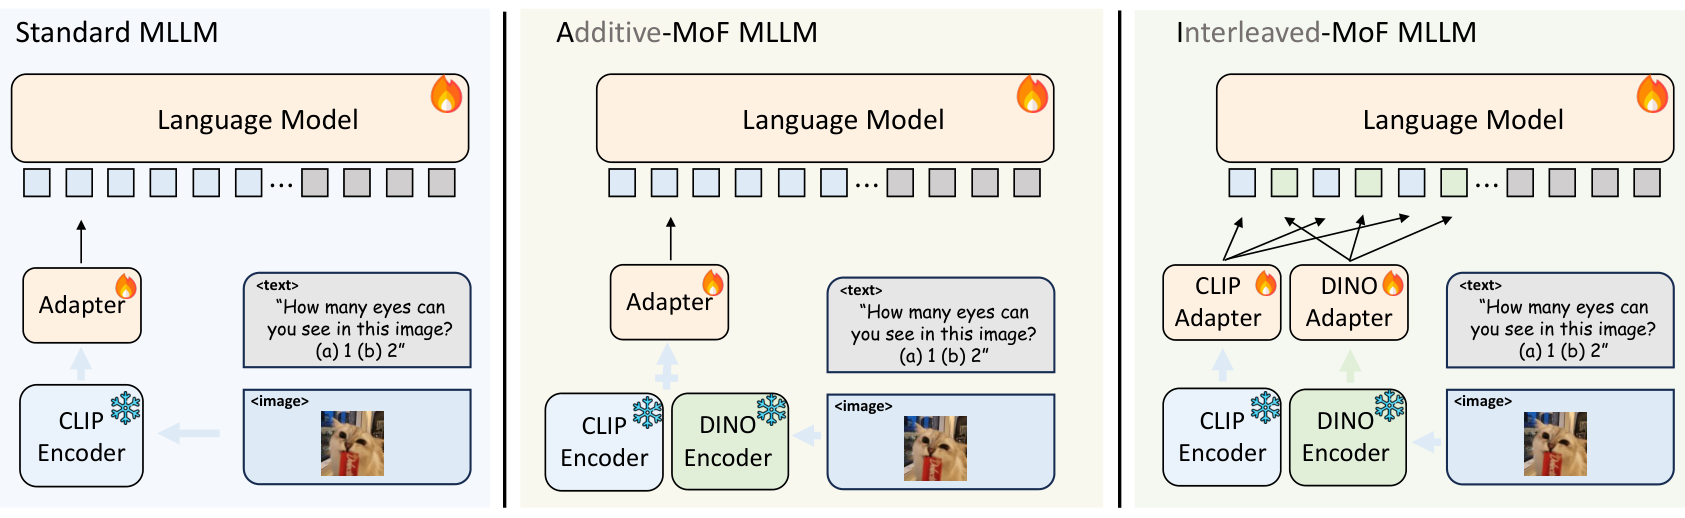
\includegraphics[width=\linewidth,height=0.38\textheight,keepaspectratio]{images/vision-language-models/mmvp_fig7_mixture_of_features.png}\\[0.2em]
  {\scriptsize Snowflake: frozen; flame: trained. Tong et al., \href{https://arxiv.org/abs/2401.06209v2}{arXiv:2401.06209v2}, Figure~7; Section~3.2, Tables~1--3 and~5.\par}
  \vspace{0.4em}
  \begin{columns}[T,onlytextwidth]
    \column{0.49\textwidth}
      \begin{itemize}\footnotesize\itemsep0.3em
        \item \textbf{Scale does not fix it:} on MMVP-VLM, where the questions become captions that CLIP must match to the right image, ten CLIP-style encoders (OpenAI CLIP, SigLIP, MetaCLIP, EVA-CLIP, and DFN, a CLIP trained on data chosen by a data filtering network) gain from more data and parameters on only 2 of the 9 patterns.
        \item \textbf{The MLLM inherits the errors:} across the nine patterns, the accuracies of CLIP and of LLaVA-1.5 correlate with Pearson $r = 0.87$.
      \end{itemize}
    \column{0.49\textwidth}
      \begin{itemize}\footnotesize\itemsep0.3em
        \item \textbf{Additive MoF} (224 px): one adapter reads $\alpha\cdot\text{CLIP} + (1-\alpha)\cdot\text{DINOv2}$. At $1-\alpha = 0.75$, MMVP rises from 5.5 to 18.7 but LLaVA-Bench drops from 81.8 to 75.8.
        \item \textbf{Interleaved MoF:} one adapter per encoder, the two token streams alternating in spatial order (224 px, 512 tokens). Against the 336-px, 576-token models: MMVP 6.0 to 16.7 (LLaVA) and 24.7 to 28.0 (LLaVA-1.5); LLaVA-Bench 81.4 to 82.8 and 84.7 to 82.7.
      \end{itemize}
  \end{columns}
\end{frame}

\begin{frame}{Language Priors: Answering Without Looking}
  \begin{columns}[T,onlytextwidth]
    \column{0.52\textwidth}
      \begin{itemize}\footnotesize\itemsep0.35em
        \item \textbf{An old problem:} on the original VQA dataset (v1), answering ``yes'' to every ``Do you see a\ldots'' question scored 87\% VQA accuracy. On balanced VQAv2 a question-only model still scores 43.01\% (best model with the image: 59.14\%).
        \item \textbf{The image is often unnecessary:} all 22 LLMs tested answer ``What is the capital of Nebraska?'' (asked over a map) blind. In ScienceQA, 57.2\% of the questions are answered blind by six or more of eight LLMs.
        \item \textbf{Leakage:} an MLLM that answers blind well above its own LLM base has probably seen the items in multimodal training (table).
        \item \textbf{Rule:} always report blind baselines, the model with the image removed (or a gray image) and its LLM alone.
      \end{itemize}
    \column{0.46\textwidth}
      \begin{itemize}\footnotesize
        \item \textbf{MMStar} keeps only samples that at most two of eight LLMs answer without the image (22,401 down to 11,607); three experts then pick 1,500 that need the image, 250 for each of six capabilities. LLMs score near random on it.
      \end{itemize}
      \vspace{0.3em}
      \centering
      {\scriptsize\setlength{\tabcolsep}{3pt}
      \begin{tabular}{l r r}
        \toprule
        MMMU validation, \% & GPT-4V & Sphinx-X-MoE \\
        \midrule
        LLM base alone, $S_t$ & 41.2 & 25.7 \\
        image removed, $S_{ov}$ & 45.1 & 43.6 \\
        with the image, $S_{wv}$ & 53.6 & 44.8 \\
        \midrule
        MG $= S_{wv} - S_{ov}$ & 8.5 & 1.2 \\
        ML $= \max(0,\, S_{ov} - S_t)$ & 3.9 & 17.9 \\
        \bottomrule
      \end{tabular}\par}
      \vspace{0.2em}
      {\scriptsize\raggedright MG, multimodal gain: what the image adds. ML, multimodal leakage: how far the blind model beats its LLM base (GPT-4 Turbo, Mixtral-8x7B). Random choice: 22.1.\par}
  \end{columns}
  \vspace{0.3em}
  {\scriptsize Goyal et al., \href{https://arxiv.org/abs/1612.00837v3}{arXiv:1612.00837v3}, Section~1, Table~1; Chen et al., ``Are We on the Right Way for Evaluating Large Vision-Language Models?,'' NeurIPS 2024, \href{https://proceedings.neurips.cc/paper_files/paper/2024/hash/2f8ee6a3d766b426d2618e555b5aeb39-Abstract-Conference.html}{proceedings.neurips.cc}, Sections~3 and~4, Figures~1, 2, 4, Tables~2, 4, Appendices~A.1 and~A.3.\par}
\end{frame}
